\documentclass[aspectratio=169, 12pt, hyperref={unicode}]{beamer}
\usepackage[utf8]{inputenc}
\usepackage[czech]{babel}
\usepackage{graphicx}
\usetheme{Madrid}
\usepackage{times}

\usepackage[euler]{textgreek}
\usepackage[font=footnotesize]{caption}


\title{Návrh pevného pozemního bezdrátového spoje}
\subtitle{B2M17SBS -- Projekt I}
\author{Šimák, Hulec, Semerád, Jína}
\date{Duben 2023}


\definecolor{cvut_navy}{HTML}{0065BD}
\definecolor{cvut_blue}{HTML}{6AADE4}
\definecolor{cvut_gray}{HTML}{156570}

\setbeamercolor{section in toc}{fg=black,bg=white}
\setbeamercolor{alerted text}{fg=cvut_blue}
\setbeamercolor*{palette primary}{bg=cvut_navy,fg=gray!20!white}
\setbeamercolor*{palette secondary}{bg=cvut_blue,fg=white}
\setbeamercolor*{palette tertiary}{parent=palette primary}
\setbeamercolor*{palette quaternary}{fg=green,bg=gray!5!white}

\setbeamercolor*{sidebar}{fg=cvut_navy,bg=gray!15!white}


\setbeamercolor{titlelike}{parent=palette primary}
\setbeamercolor{frametitle}{parent=palette primary}

\setbeamercolor*{separation line}{}
\setbeamercolor*{fine separation line}{}

\setbeamertemplate{navigation symbols}{} 

\setbeamercolor{itemize item}{fg=cvut_blue}
\setbeamercolor{itemize subitem}{fg=cvut_blue}
\setbeamercolor{itemize subsubitem}{fg=cvut_blue}
\setbeamercolor{section number projected}{bg=cvut_navy}
\setbeamercolor{caption name}{fg=cvut_blue}

\setbeamertemplate{itemize item}[circle]
\setbeamertemplate{itemize subitem}[circle]
\setbeamertemplate{itemize subsubitem}[circle]
\setbeamertemplate{caption}[numbered]

\begin{document}

\logo{
\includegraphics[height=1cm]{src/symbol_cvut_plna_samostatna_verze.pdf}}

\begin{frame}
\titlepage
\end{frame}

\begin{frame}
\frametitle{Obsah}
\tableofcontents
\end{frame}

\section{Zadání}
\begin{frame}
\frametitle{Zadání}
\begin{itemize}
\item Návrh řešení mikrovlnného spoje pro vysokokapacitní přenos dat
\item FEL ČVUT v Praze, Technická 2 (50,103153N; 14,392759E; maximální možná
výška umístění antény 40 m nad zemí)
\item  Fiktivní odloučené pracoviště v Berouně s anténou na rozhledně na Městské hoře (49,9626386N; 14,0650983E; výška 14 m nad terénem)
\item Dostupnost spoje: 99,99\% pro BER 10-6
\end{itemize}
\end{frame}

\section{Trasa spoje}
\begin{frame}
\frametitle{Trasa spoje}
\begin{columns}
\begin{column}{0.5\textwidth}
    \begin{figure}[!ht]
        \centering
        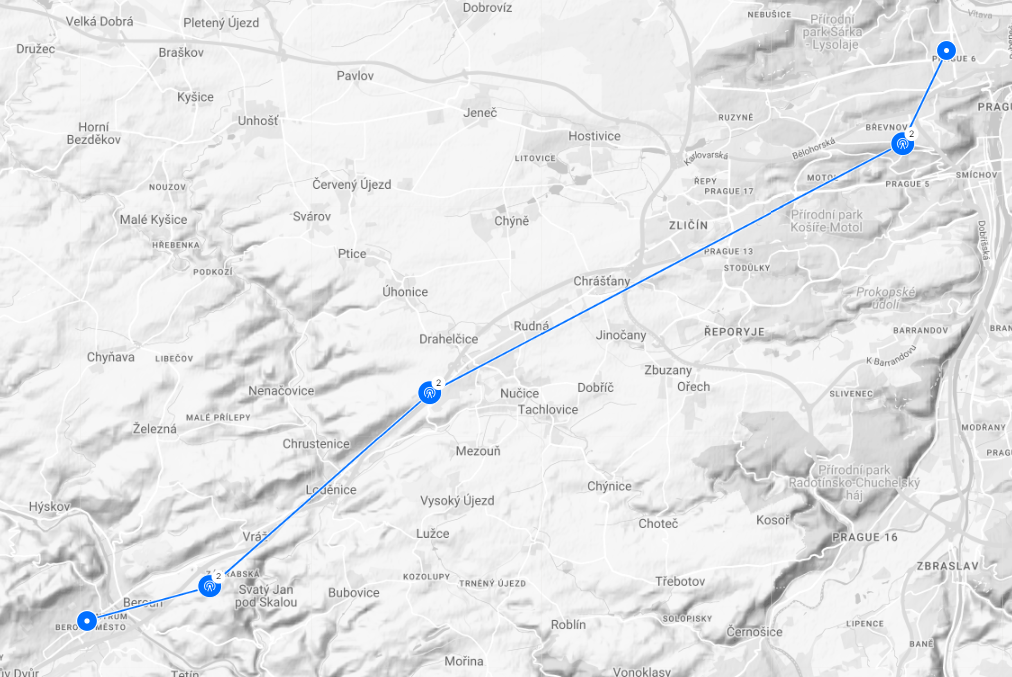
\includegraphics[width=\textwidth]{src/mapa.png}
    \end{figure}
\end{column}
\begin{column}{0.5\textwidth}
\begin{itemize}
\vspace{-1.5cm}
\item Budova FEL, ČVUT v Praze, Technická 2
\item Vysílač Strahov
\item Vysílač Rudná
\item Vysílač Beroun-Závodí
\item Rozhledna Městská hora, Beroun-Město
\end{itemize}
\end{column}
\end{columns}
\end{frame}

\begin{frame}
\frametitle{FEL -- Strahov}
\begin{figure}[!ht]
	\begin{center}
		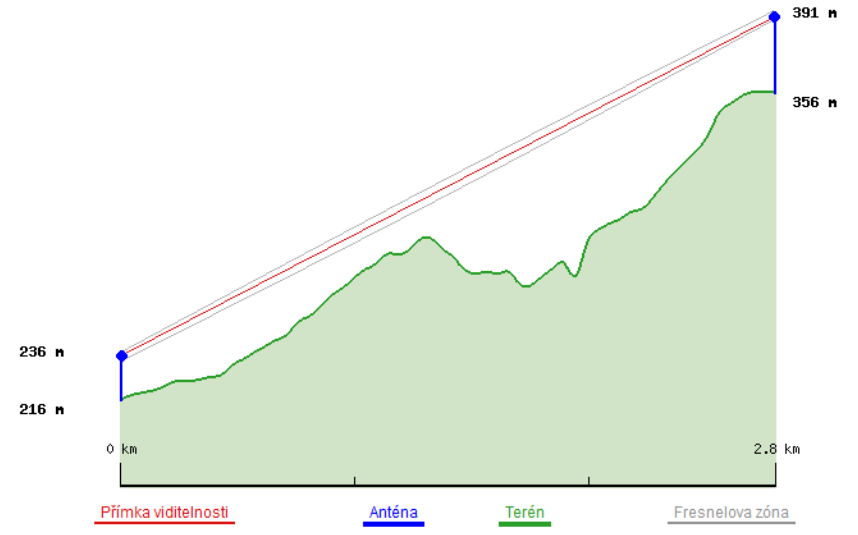
\includegraphics[width=.7\textwidth]{src/fel-strahov.png}
	\end{center}
\end{figure}
\end{frame}

\begin{frame}
\frametitle{Strahov -- Rudná}
\begin{figure}[!ht]
	\begin{center}
		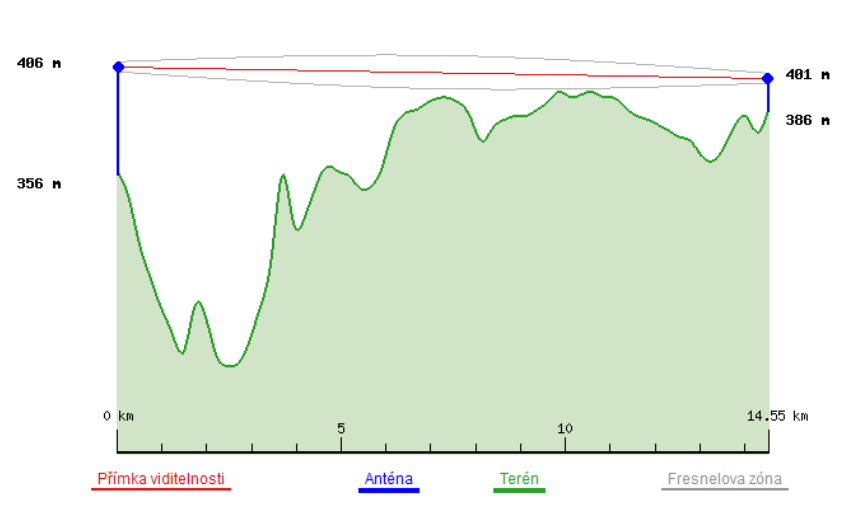
\includegraphics[width=.7\textwidth]{src/strahov-rudna.png}
	\end{center}
\end{figure}
\end{frame}

\begin{frame}
\frametitle{Rudná -- Závodí}
\begin{figure}[!ht]
	\begin{center}
		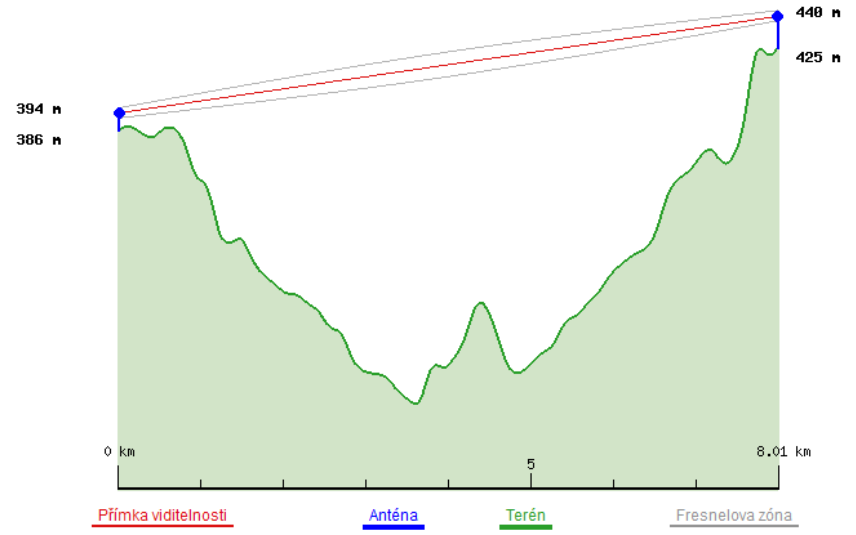
\includegraphics[width=.7\textwidth]{src/rudna-zavodi.png}
	\end{center}
\end{figure}
\end{frame}

\begin{frame}
\frametitle{Závodí -- Beroun}
\begin{figure}[!ht]
	\begin{center}
		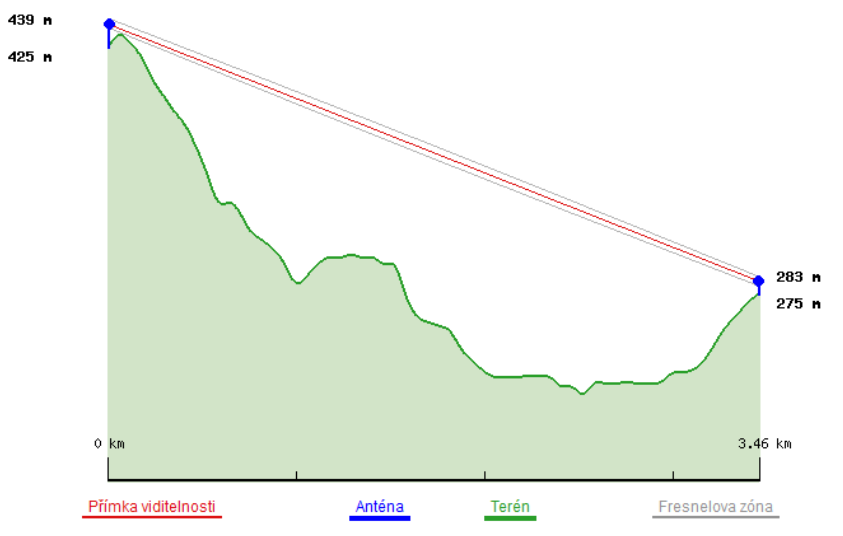
\includegraphics[width=.7\textwidth]{src/zavodi-beroun.png}
	\end{center}
\end{figure}
\end{frame}

\begin{frame}
\frametitle{Parametry cest}
\begin{table}[h!]
\scalebox{0.8}{
\begin{tabular}{| l || c | c | c | c |}
    \hline
    & FEL -- Strahov & Strahov -- Rudná & Rudná -- Závodí & Závodí -- Beroun\\
    \hline\hline
    $d \; [\text{km}]$ & 2.81 & 14.57 & 8.02 & 3.47\\
    \hline
    $F1 \; [\text{m}]$ & 1.25 & 7.31 & 1.28 & 1.27\\
    \hline			
    $x \; [\text{m}]$ & 0.02 & 3.38 & 0.06 & 0.02\\
    \hline
    $Txh \; [\text{m}]$ & 20 & 50 & 8 & 14\\
    \hline
    $Rxh \; [\text{m}]$ & 10 & 20 & 10 & 5\\
    \hline
\end{tabular}}
\end{table}
\[\begin{array}{lll}
    d &\quad& \text{Délka spoje}\\
    x &\quad& \text{Maximální chyba způsobená zakřivením Země}\\
    F1 &\quad& \text{Poloměr 1. Fresnelovy zóny}\\
    Txh &\quad& \text{Výška vysílací antény}\\
    Rxh &\quad& \text{Výška přijímací antény}
\end{array}\]
\end{frame}

\section{Volba antén}
\begin{frame}
\frametitle{Volba antén}
\begin{columns}
\begin{column}{0.5\textwidth}
\begin{table}[ht]
		\centering
		\scalebox{0.8}{
		\begin{tabular}[t]{|l || c | c |}
            \hline
            Spoj & Průměr & Zisk\\
			\hline\hline
			FEL -- Strahov & 0.3 m & 33 dBi\\   
			\hline
			Strahov -- Rudná & 0.9 m & 42 dBi\\
			\hline
			Rudná -- Závodí & 0.6 m & 38.5 dBi\\
			\hline
			Závodí -- Beroun & 0.3 m & 33 dBi\\
			\hline
		\end{tabular}}
	\end{table}%\\
\end{column}
\begin{column}{0.5\textwidth}
ALCOMA AL18F
\begin{itemize}
    \item Pracovní frekvence: $18 \; \text{GHz}$
    \item Modulační schéma: 256QAM
    \item Šířka pásma: $55 \; \text{MHz}$
    \item Přenosová kapacita: $376 \; \text{Mbps}$
    \item Maximální výstupní výkon: $17 \; \text{dBm}$
    \item Polarizace: vertikální
\end{itemize}
\end{column}
\end{columns}
\end{frame}

\section{Výkonová bilance}
\begin{frame}
\frametitle{Výkonová bilance}
\begin{table}[ht]
	\centering
	\scalebox{1}{
		\begin{tabular}[t]{|l||c|c|c|c|}
			\hline
			Úsek & $P_t \; [\text{dBm}]$ & $L_{\text{gas}} \; [\text{dB}]$ & $\text{FSL} \; [\text{dB}]$ & Rezerva$\; [\text{dB}]$ \\   
			\hline\hline
			FEL -- Strahov & 10 & 0.17 & 126.52 & 13.31\\
			\hline
			Strahov -- Rudná & 17 & 0.87 & 140.82 & 23.31\\
			\hline
			Rudná -- Závodí & 15 &  0.48 & 135.63 & 19.89\\
			\hline
			Závodí -- Beroun & 12 & 0.21 & 128.36 & 13.43\\
            \hline
		\end{tabular}}
	\end{table}
\end{frame}

\begin{frame}
\frametitle{Úniky}
\begin{table}[ht]
		\centering	
		\begin{tabular}[t]{|l||c|}
			\hline
			Spoj & $pw \; [\text{\%}]$\\
			\hline\hline
			FEL -- Strahov & 4.59$\cdot$10\textsuperscript{-6}\\  
			\hline
			Strahov -- Rudná & 5.8$\cdot$10\textsuperscript{-4}\\
			\hline
			Rudná -- Závodí & 6.6$\cdot$10\textsuperscript{-5}\\
			\hline
			Závodí -- Beroun & 8.45$\cdot$10\textsuperscript{-6}\\
			\hline
		\end{tabular}
	\end{table}
	\begin{itemize}
		\item $p_{\text{multihop}} = 6.4 \cdot 10^{-4} \; \text{\%}$
	\end{itemize}
\end{frame}

\begin{frame}
\frametitle{Útlum deštěm}
	\begin{table}[h!]
		\centering
		\begin{tabular}{| l || c | c | c |}
			\hline
			Spoj & $d_{\text{eff}} \; [\text{m}]$ & $A_{0.01} \; [\text{dB}]$ & $p_{\mathrm{rain}} \; [\%]$\\
			\hline\hline
			FEL -- Strahov & 2.9 & 6.8 & $3.4 \cdot 10^{-4}$\\
			\hline
			Strahov -- Rudná & 9.24 & 21.66 & $4.5 \cdot 10^{-4}$\\
			\hline
			Rudná -- Závodí & 5.87 & 13.75 & $3.9 \cdot 10^{-4}$\\
			\hline
			Závodí -- Beroun & 3.31 & 7.76 & $3.6 \cdot 10^{-4}$\\
			\hline
		\end{tabular}
	\end{table}
	\begin{itemize}
		\item $R_{0.01} = 25.42 \;\text{mm/h}$
		\item $\gamma_R = 2.34 \;\text{dB/km}$
	\end{itemize}
\end{frame}

\setbeamercolor{background canvas}{bg=white}

\end{document}
